\begin{frame}\frametitle{Large Hadron Collider (LHC)}
  \begin{figure}[htb]
    \begin{center}
      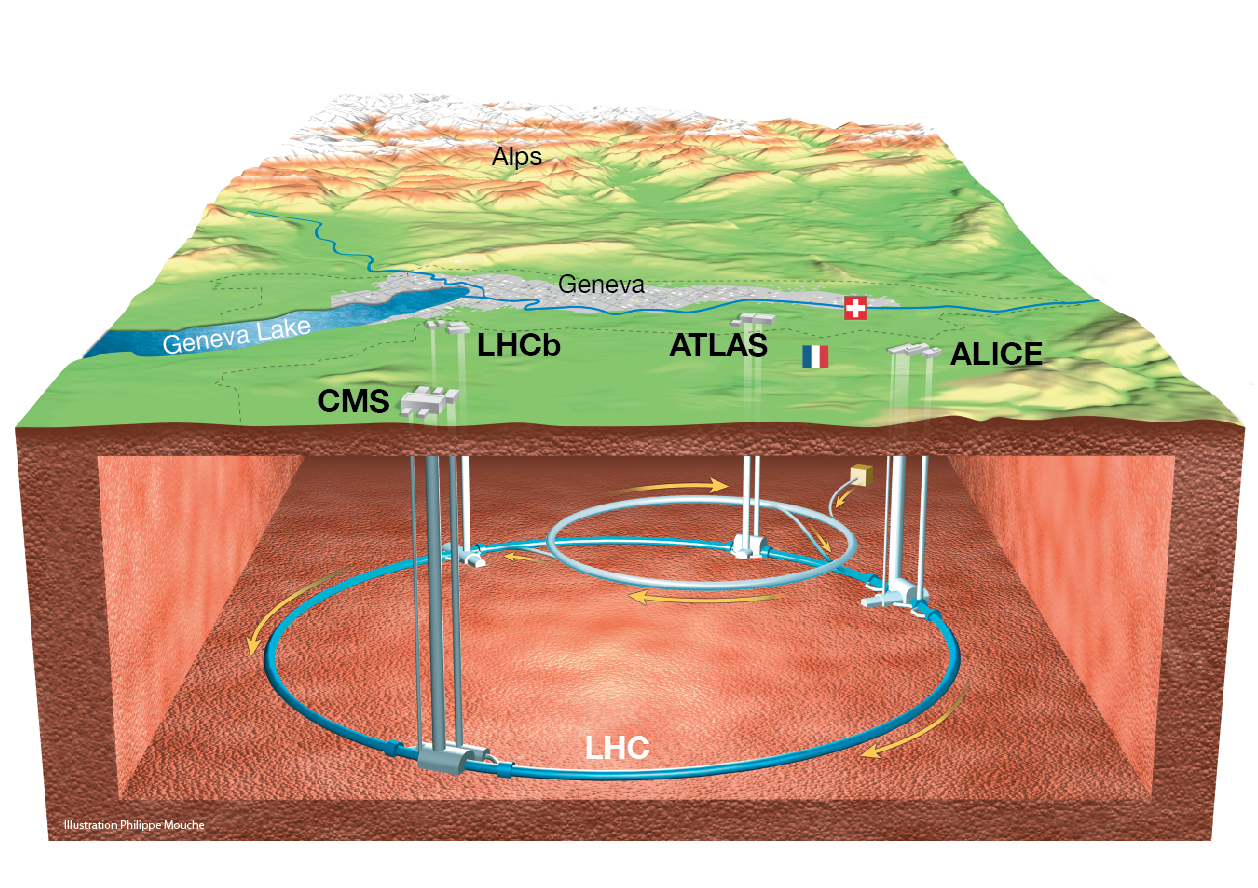
\includegraphics[width=0.80\textwidth]{../figs/ForPresentation/LHC.png}
    \end{center}
  \end{figure}
\tiny
http://lhcathome.web.cern.ch/about
\end{frame}%{Large Hadron Collider}

\begin{frame}\frametitle{Compact Muon Solenoid (CMS)}
\begin{figure}[htb]
  \begin{center}
    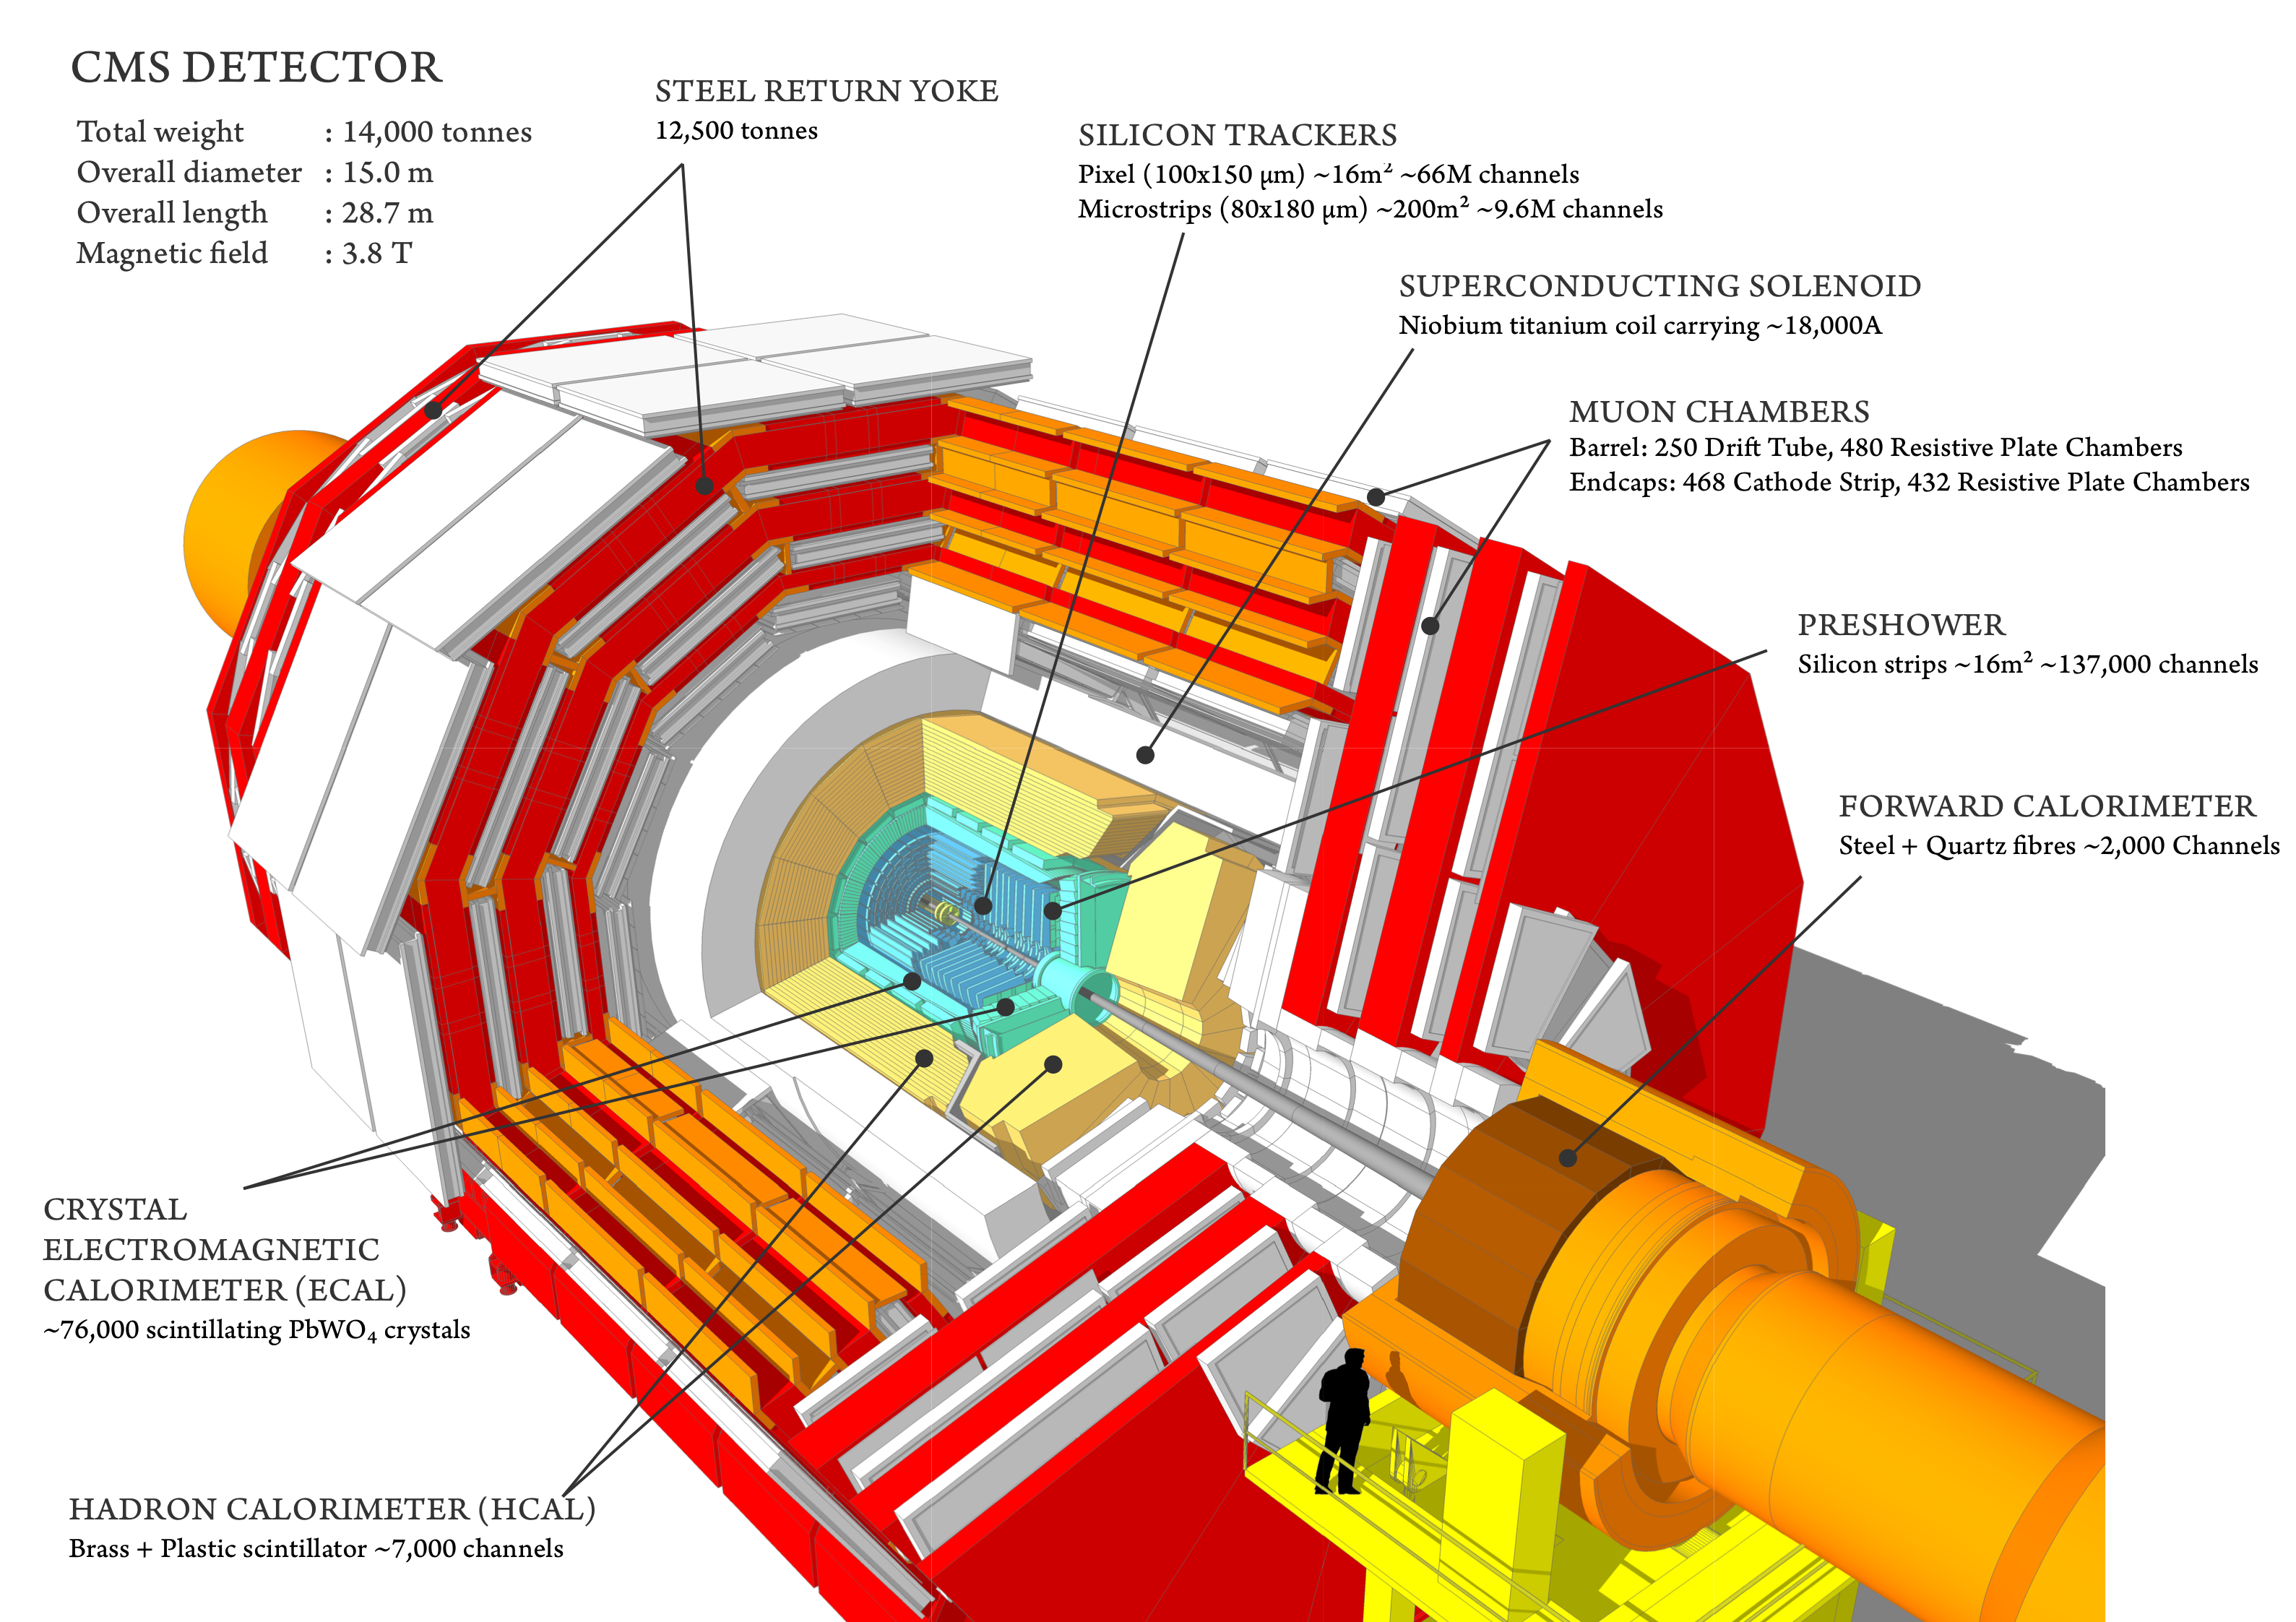
\includegraphics[width=0.90\textwidth]{../figs/ForPresentation/CMS.png}
  \end{center}
\end{figure}
\tiny
http://cms.web.cern.ch/news/cms-detector-design
\end{frame}%{Compact Muon Solenoid (CMS). Components}


\begin{frame}\frametitle{Compact Muon Solenoid (CMS). Particle Reconstruction}
\tiny
Process to study: $W\gamma\rightarrow\mu\nu\gamma$, $W\gamma\rightarrow e\nu\gamma$.\\
\definecolor{celestialblue}{rgb}{0.29, 0.59, 0.82}
\definecolor{egyptianblue}{rgb}{0.06, 0.2, 0.65}
Final state particles: {\color{celestialblue}{muons}}, {\color{red}electrons}, {\color{egyptianblue}photons}, neutrinos.\\
\begin{figure}[htb]
  \begin{center}
    {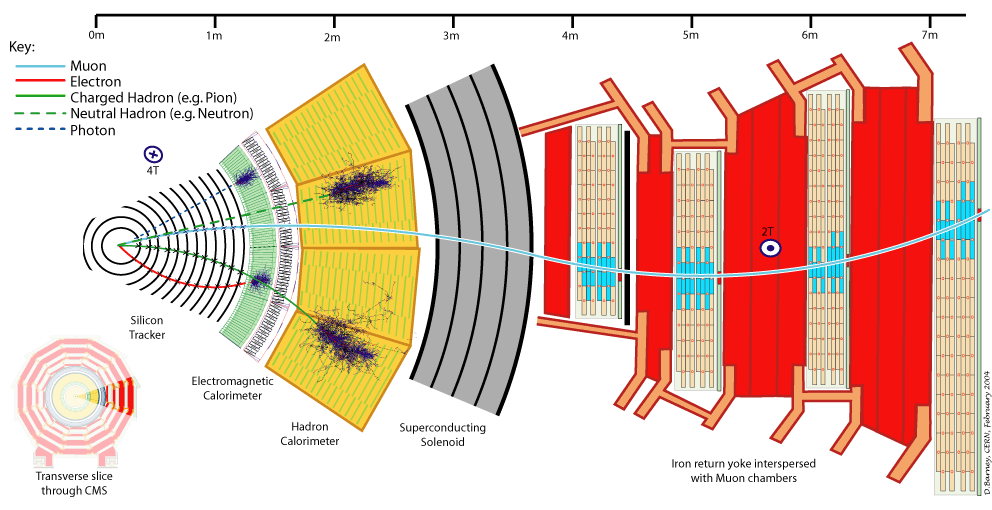
\includegraphics[width=0.98\textwidth]{../figs/ForPresentation/CMS_Slice.png}}
  \end{center}
\end{figure}

\tiny
Neutrino is not detected. \\
The measure of $P_T^{\nu}$ is missing transverse energy: $  E_T^{miss} = - | \sum \mathbf{P_T} |$. (Sum over all detected particles).\\

\end{frame}%{Compact Muon Solenoid (CMS). Particle Reconstruction}


